\documentclass[12pt, twoside]{article}
%\documentclass[12pt, twoside]{article}
\usepackage[letterpaper, margin=1in, headsep=0.2in]{geometry}
\setlength{\headheight}{0.6in}
%\usepackage[english]{babel}
\usepackage[utf8]{inputenc}
\usepackage{microtype}
\usepackage{amsmath}
\usepackage{amssymb}
%\usepackage{amsfonts}
\usepackage[nomessages]{fp} %\FPeval{\var-name}{2*sin(pi/6)}
\usepackage{siunitx} %units in math. eg 20\milli\meter
\usepackage{yhmath} % for arcs, overparenth command
\usepackage{tikz} %graphics
\usetikzlibrary{quotes, angles, arrows, arrows.meta}
\usepackage{pgfplots}
\usepgfplotslibrary{fillbetween}
\pgfplotsset{compat=1.16}
\usepackage{graphicx} %consider setting \graphicspath{{images/}}
\usepackage{parskip} %no paragraph indent
\usepackage{enumitem}
\usepackage{multicol}
\usepackage{venndiagram}

\usepackage{fancyhdr}
\pagestyle{fancy}
\fancyhf{}
\renewcommand{\headrulewidth}{0pt} % disable the underline of the header
\raggedbottom
\hfuzz=2mm %suppresses overfull box warnings

\usepackage{hyperref}

\fancyhead[LO]{La Scuola d'Italia / Dr.\ Huson / IB Math 11 \\* 4 November 2026}
\fancyhead[RO]{\fbox{\begin{minipage}{6cm}\footnotesize Nickname:\\[0.5cm]\end{minipage}}}
\fancyfoot[C]{\thepage}

\newcommand{\ita}[1]{(\emph{#1})}

\begin{document}
\subsubsection*{2.9 Classwork: Every Rate of Change Has a Name}

In every field, the slope \ita{pendenza, coefficiente angolare} of a line
gets its own name, and the intercept \ita{intercetta, ordinata
all'origine} means something too. These models show how things work, but
real life is more complicated. All figures are simplified.

%--- Example 1: NYC sales tax, direct proportion; inverse (price before tax) ---
%--- Source: Original (AA SL 2.1, 2.2) ---
\textbf{1. Sales tax in New York City.} The sales tax rate \ita{aliquota}
is $8.875\%$. For a price $x$ dollars before tax, the amount paid is
$P = 1.08875x$. The graph is a line through the origin: a direct
proportion \ita{proporzionalità diretta}. Its slope, $1.08875$, is the
constant of proportionality \ita{costante di proporzionalità}.

\begin{enumerate}[label=(\alph*), itemsep=0.1cm]
  \item A receipt shows a total of $\$174.20$. Find the price before tax.
  \vspace{1.4cm}
\end{enumerate}

%--- Example 2: Simplified income tax T = 0.12(I - 16000): marginal rate, deduction as x-intercept, average rate curve, credit vs deduction as shifts ---
%--- Source: Original (AA SL 2.1, 2.11); simplified from 2026 US federal rules ---
\textbf{2. Income tax, one bracket.}

\begin{minipage}[t]{0.5\linewidth}
Simplified US model: no tax on the first $\$16\,000$ of income (the
standard deduction \ita{deduzione standard}), then $12\%$ on the rest.
\[
  T = 0.12(I - 16\,000), \quad I \ge 16\,000.
\]
The slope, $0.12$, is the \textbf{marginal tax rate} \ita{aliquota
marginale}: the tax on one more dollar. The deduction is the
$I$-intercept, not the $T$-intercept.
\end{minipage}
\hfill
\begin{minipage}[t]{0.46\linewidth}
\vspace{0pt}
\begin{tikzpicture}
\begin{axis}[
  axis lines=left,
  xlabel={$I$ (\$1000)}, ylabel={$T$ (\$1000)},
  xlabel style={at={(axis description cs:1,0)}, anchor=north east, yshift=-0.5cm, font=\footnotesize},
  ylabel style={at={(axis description cs:0,1)}, anchor=south, rotate=-90, font=\footnotesize},
  xmin=0, xmax=60, ymin=0, ymax=6,
  xtick={0,16,40,60}, ytick={0,2,4,6},
  tick label style={font=\footnotesize},
  width=6.8cm, height=4.6cm, clip=false,
]
  \addplot[very thick, domain=16:60] {0.12*(x-16)};
  \addplot[only marks, mark=*, mark size=1.5pt] coordinates {(16,0)};
  \draw[dashed] (axis cs:40,2.88) -- (axis cs:50,2.88) -- (axis cs:50,4.08);
  \node[font=\scriptsize, anchor=west] at (axis cs:50,3.4) {rise $1.2$};
  \node[font=\scriptsize, anchor=north] at (axis cs:45,2.85) {run $10$};
\end{axis}
\end{tikzpicture}
\end{minipage}

\begin{enumerate}[label=(\alph*), itemsep=0.1cm]
  \item Find the tax on an income of $\$40\,000$.
  \vspace{1.1cm}
  \item The \textbf{average tax rate} \ita{aliquota media} is $T \div I$.
  Find it for $I = 40\,000$ and for $I = 100\,000$. Will it ever reach
  $12\%$? Is the graph of the average rate a straight line?
  \vspace{1.8cm}
  \item A \emph{tax credit} \ita{credito d'imposta, detrazione} of $\$500$
  subtracts $500$ from $T$. A larger deduction of $\$20\,000$ replaces
  $16\,000$. Describe how each one moves the graph.
  \vspace{1.6cm}
\end{enumerate}

\newpage

%--- Example 3: Budget line 3x + 4y = 24, negative slope = relative price / opportunity cost ---
%--- Source: Original (AA SL 2.1) ---
\textbf{3. A budget line \ita{vincolo di bilancio} on Mulberry Street.}
You have $\$24$ to spend on espressos at $\$3$ and cannoli at $\$4$. With
$x$ espressos and $y$ cannoli, $3x + 4y = 24$. The slope is
$-\frac{3}{4}$, a \textbf{negative} rate of change: each extra espresso
costs $\frac{3}{4}$ of a cannolo. This is the relative price
\ita{prezzo relativo}, or opportunity cost \ita{costo opportunità}.

\begin{enumerate}[label=(\alph*), itemsep=0.1cm]
  \item Find both intercepts and say what each one means.
  \vspace{1.1cm}
  \item The price of a cannolo rises to $\$6$. Write the new budget line
  and find its slope.
  \vspace{1.1cm}
\end{enumerate}

%--- Example 4: Pizzeria break-even: C = 9000 + 6q, R = 18q; marginal cost, contribution margin, break-even ---
%--- Source: Original (AA SL 2.1 systems) ---
\textbf{4. Break-even at an Arthur Avenue pizzeria.} Fixed costs
\ita{costi fissi} are $\$9000$ a month. Each pizza costs $\$6$ to make and
sells for $\$18$. For $q$ pizzas a month, cost is $C = 9000 + 6q$ and
revenue \ita{ricavo} is $R = 18q$. The slope of $C$ is the
\textbf{marginal cost} \ita{costo marginale}. The slope of the profit
$R - C$ is the \textbf{contribution margin} \ita{margine di
contribuzione}.

\begin{enumerate}[label=(\alph*), itemsep=0.1cm]
  \item Find the break-even point \ita{punto di pareggio}, where $C = R$.
  \vspace{1.1cm}
  \item Find the profit when the pizzeria sells $1000$ pizzas in a month.
  \vspace{1.1cm}
\end{enumerate}

%--- Example 5: Tariff on Italian cheese: demand p = 40 - 2q, supply p = 16 + q; $3/kg tariff shifts supply up; pass-through 2/3 ---
%--- Source: Original (AA SL 2.1 systems, 2.11 translation); 2025 US tariff on EU goods, simplified ---
\textbf{5. A tariff \ita{dazio} on imported Parmigiano.} In the US market,
demand is $p = 40 - 2q$ and supply is $p = 16 + q$, where $p$ is dollars per
kg and $q$ is thousand kg per week. The demand slope, $-2$, is the
\textbf{price sensitivity} \ita{sensibilità al prezzo}. (Economists also
use \emph{elasticity} \ita{elasticità}: the same idea in percent terms,
\% change in quantity per \% change in price.)

\begin{enumerate}[label=(\alph*), itemsep=0.1cm]
  \item Use elimination to find the equilibrium quantity and price.
  \vspace{1.2cm}
  \item A tariff of $\$3$ per kg shifts the supply line up by $3$. Find the
  new equilibrium.
  \vspace{1.2cm}
  \item How much of the $\$3$ tariff do buyers pay? This share is the
  \textbf{pass-through} \ita{traslazione dell'imposta}.
  \vspace{0.8cm}
\end{enumerate}

\newpage

%--- Example 6: Flat-rate tax vs standard tax for a freelancer: 0.15R vs 0.25(R - 20000); break-even revenue 50000 ---
%--- Source: Original (AA SL 2.1 systems); idea from Italy's regime forfettario, simplified ---
\textbf{6. Two ways to pay tax.} Some countries, Italy among them
\ita{regime forfettario}, let a freelancer choose a flat-rate tax on
revenue. Simplified, for revenue $R$ dollars:

\smallskip
\begin{tabular}{@{}ll@{}}
  Flat rate: & $T = 0.15R$ \quad (slope: the \textbf{effective rate} \ita{aliquota effettiva}) \\
  Standard: & $T = 0.25(R - 20\,000)$ \quad (slope: the marginal rate)
\end{tabular}

\begin{enumerate}[label=(\alph*), itemsep=0.1cm]
  \item Use elimination to find the revenue at which the two options cost
  the same. Which option is cheaper for $R = 80\,000$?
  \vspace{1.6cm}
\end{enumerate}

%--- Example 7: Stock beta: r = alpha + beta r_m; bank (beta 1.5), utility (beta 0.5), inverse ETF (beta -1); portfolio mix to beta 1.2 ---
%--- Source: Original (AA SL 2.1 systems); simplified one-factor model ---
\textbf{7. Stocks and the market.} A simple model links a stock's monthly
return \ita{rendimento} $r$ to the market's return $r_m$ (both in \%):
$r = \alpha + \beta\, r_m$. The slope $\beta$ is the \textbf{beta}
\ita{coefficiente beta}: how many \% the stock moves per $1\%$ move of the
market. The intercept $\alpha$ \ita{alfa} is the return when the market is
flat.

\begin{tabular}{@{}lll@{}}
  A bank stock: & $r = 0.5 + 1.5\,r_m$ & \\
  Con Edison (a utility): & $r = 0.2 + 0.5\,r_m$ & \\
  An inverse fund \ita{ETF inverso}: & $r = -r_m$ & ($\beta = -1$: a \textbf{negative} slope)
\end{tabular}

\begin{enumerate}[label=(\alph*), itemsep=0.1cm]
  \item The market falls $4\%$ in a month. Find the return on each of the
  three.
  \vspace{1.2cm}
  \item You split $\$10\,000$ between the bank ($\$x$) and Con Edison
  ($\$y$) so that the portfolio has a beta of $1.2$:
  $1.5x + 0.5y = 1.2 \times 10\,000$. Find $x$ and $y$.
  \vspace{1.6cm}
\end{enumerate}

%--- Example 8: Bond duration: P ~ 100 - 7(y - 4); two-bond portfolio with durations 2 and 7 to target duration 5 ---
%--- Source: Original (AA SL 2.1 systems); simplified duration model ---
\textbf{8. Bonds \ita{obbligazioni}: price falls when yield rises.} When
interest rates (yields, \ita{rendimento a scadenza}) rise, the price of a
bond falls: a \textbf{negative} slope. The \textbf{duration}
\ita{durata finanziaria} is that slope in percent terms: a duration of
$7$ means the price falls about $7\%$ when the yield rises by $1$
percentage point. For a US Treasury bond priced at $\$100$ when the yield
is $4\%$: $P \approx 100 - 7(y - 4)$, with $y$ in \%.

\begin{enumerate}[label=(\alph*), itemsep=0.1cm]
  \item Estimate the price if the yield rises to $4.5\%$.
  \vspace{0.9cm}
  \item You split $\$100\,000$ between a short bond (duration $2$) and a
  long bond (duration $7$) to get a duration of $5$:
  $2x + 7y = 5 \times 100\,000$. Find the amount in each bond.
  \vspace{1.4cm}
\end{enumerate}

\newpage

\textbf{When the rate of change changes: curves.} In Example 2(b) the
average tax rate was not a straight line. When the slope itself changes,
we need curves. The way the slope changes also has a name.

%--- Example 9: Bond convexity: zero-coupon P = 100/(1 + y)^10 vs tangent line at 4% ---
%--- Source: Original (AA SL 1.4 compound interest, 2.4 graphs); convexity preview ---
\textbf{9. Convexity \ita{convessità}.} A 10-year zero-coupon bond pays
$\$100$ in 10 years. Its price is the present value
$P = \dfrac{100}{(1 + y/100)^{10}}$, where $y$ is the yield in \%. The
straight line is the duration estimate at $4\%$:
$L = 67.56 - 6.50(y - 4)$.

\begin{minipage}[t]{0.47\linewidth}
\vspace{0pt}
\renewcommand{\arraystretch}{1.3}
\begin{tabular}{|c|c|c|}
  \hline
  Yield (\%) & Price $P$ & Line $L$ \\ \hline
  $2$ & & $80.55$ \\ \hline
  $3$ & & $74.05$ \\ \hline
  $4$ & $67.56$ & $67.56$ \\ \hline
  $5$ & & $61.06$ \\ \hline
  $6$ & & $54.56$ \\ \hline
\end{tabular}
\end{minipage}
\hfill
\begin{minipage}[t]{0.5\linewidth}
\vspace{0pt}
\begin{tikzpicture}
\begin{axis}[
  axis lines=left,
  xlabel={yield (\%)}, ylabel={price},
  xlabel style={font=\footnotesize, yshift=0.15cm},
  ylabel style={font=\footnotesize, yshift=-0.2cm},
  xmin=1.5, xmax=6.5, ymin=50, ymax=85,
  xtick={2,3,4,5,6}, ytick={50,55,...,85},
  grid=major, grid style={line width=0.2pt, gray!40},
  tick label style={font=\footnotesize},
  width=7.4cm, height=5.4cm,
]
  \addplot[thick, dashed, domain=1.7:6.3] {67.56 - 6.50*(x-4)};
  \node[font=\scriptsize, fill=white, inner sep=1pt] at (axis cs:5.9,59.0) {$L$};
  % solution curve (MS check):
  %\addplot[very thick, domain=1.7:6.3, samples=60] {100/(1+x/100)^10};
\end{axis}
\end{tikzpicture}
\end{minipage}

\begin{enumerate}[label=(\alph*), itemsep=0.1cm]
  \item Use your GDC to complete the table. Plot the prices and join them
  with a smooth curve.
  \item Is the curve above or below the line? Does the curve get steeper or
  less steep as the yield rises?
  \vspace{0.9cm}
\end{enumerate}

%--- Example 10: Learning curve: cost per unit x0.8 per doubling from $10000; economies of scale ---
%--- Source: Original (AA SL 1.3 geometric sequences); Wright's law, simplified ---
\textbf{10. Economies of scale \ita{economie di scala}: the learning curve
\ita{curva di apprendimento}.} A factory's first battery pack costs
$\$10\,000$. Each time the number of packs made doubles, the cost per
pack falls by $20\%$ (the \textbf{learning rate}).

\begin{enumerate}[label=(\alph*), itemsep=0.1cm]
  \item Find the cost of pack number $2$, $4$, $8$, $16$ and $32$. Which
  pack is the first to cost less than $\$4500$?
  \vspace{1.2cm}
\end{enumerate}

%--- Example 11: Logistic adoption: S-curve, first and second differences, inflection point ---
%--- Source: Original (AA SL 2.4 key features); simplified adoption data ---
\textbf{11. The S-curve \ita{curva logistica}.} Percent of US households
owning a new product, $t$ years after launch (simplified):

\begin{center}
\renewcommand{\arraystretch}{1.3}
\begin{tabular}{|l|c|c|c|c|c|c|c|c|c|}
  \hline
  $t$ & 0 & 1 & 2 & 3 & 4 & 5 & 6 & 7 & 8 \\ \hline
  \% & 2 & 5 & 12 & 27 & 50 & 73 & 88 & 95 & 98 \\ \hline
  1st difference & \multicolumn{9}{c|}{} \\ \hline
\end{tabular}
\end{center}

\begin{enumerate}[label=(\alph*), itemsep=0.1cm]
  \item Complete the first differences. When is the product spreading
  fastest? This is the \textbf{inflection point} \ita{punto di flesso},
  where the curve changes from bending up to bending down.
  \vspace{0.6cm}
\end{enumerate}

\end{document}
